\documentclass[main.tex]{subfiles}
\begin{document}

\setcounter{footnote}{0} 

\chapter{Theoretical Background}

\section{Electronic Structure}
\subsection{Preamble}
Electronic structure theory plays a pivotal role in much of computational chemistry, providing energies and derivatives of the energy that can be used to predict and rationalise experimental observations. In particular, the solution of the time-independent Schr\"{o}edinger equation,
\begin{equation}
\hat{H} \Psi  = E \Psi
\label{tise}
\vspace{-0.3cm}
\end{equation}
is sought; where $\hat{H}$ is the system's Hamiltonian describing the kinetic and potential energies of all particles described by the wave function ($\Psi$) with  energy ($E$). Unfortunately, Eqn. \eqref{tise} is insoluble for all but the most simple Hamiltonians; thus a series of approximations are therefore applied to reach a tractable problem for most chemical systems.

For polyatomic systems it is usually necessary to make the Born-Oppenheimer approximation, such that there is no coupling between electronic and nuclear wave functions, i.e. $\Psi = \psi(\boldsymbol{r}; \boldsymbol{R})\phi(\boldsymbol{R})$, for electronic coordinates $\boldsymbol{r}$ and nuclear coordinates $\boldsymbol{R}$. The Hamiltonian is then,
\begin{equation}
\hat{H}_\text{elec} = \hat{T}_\text{elec} + \hat{V}_\text{elec-nuc} + \hat{V}_\text{elec-elec} +  \hat{V}_\text{nuc-nuc}
\end{equation}
which, in first quantisation is,
\begin{equation}
\hat{H}_\text{elec} = -\frac{1}{2}\sum_{i}^\text{elec} \nabla^2_i  - \sum_{i}^\text{elec}\sum_A^\text{nuc}\frac{Z_A}{|\boldsymbol{r}_i - \boldsymbol{R}_A|} +  \sum_{i}^\text{elec}\sum_{j < i}^\text{elec} \frac{1}{|\boldsymbol{r}_i - \boldsymbol{r}_j|} + \sum_{A}^\text{nuc}\sum_{B < A}^\text{nuc} \frac{Z_A Z_B}{|\boldsymbol{R}_A - \boldsymbol{R}_B|}
\label{H_elec}
\end{equation}
 in atomic units, with nuclear charges $Z_A$ and $\nabla$ is the Laplacian operator and the final term is just a constant with respect to the electronic wave function $\hat{V}_\text{nuc-nuc} = V_\text{nn}$. With an electronic Hamiltonian the ground sate energy may be obtained using the variational principle,
 \begin{equation}
 	E_\text{est.} = \min_{\{\alpha\}}\left(\frac{\braket{\psi(\alpha) | \hat{H}_\text{elec}| \psi(\alpha)}}{\braket{\psi(\alpha)| \psi(\alpha)}}\right) \ge E_0
 \end{equation}
 
 for the best estimate of the energy given a wavefunction in parameters $\alpha$, which is guaranteed to be higher or equal to the true ground state energy ($E_0$).

\subsection{Hartree Fock}

Given Eqn. \eqref{tise} with the electronic Hamiltonian [Eqn. \eqref{H_elec}] is only analytically soluble for one-electron systems, e.g. the hydrogen atom, an approximate solution is required for poly-electron systems. Hartree-Fock (HF) theory is one such approximation and makes use of a wave function ansatz built from hydrogen-like electron eigenfunctions (orbitals), which to enforce antisymmetry, may be written as a Slater determinant,

\begin{equation}
\psi_\text{HF}(\boldsymbol{r}) = \frac{1}{n!}
\begin{vmatrix}
\varphi_1(\boldsymbol{r}_1) & \varphi_2(\boldsymbol{r}_1) & \varphi_3(\boldsymbol{r}_1) & \cdots \\
\varphi_1(\boldsymbol{r}_2) & \varphi_2(\boldsymbol{r}_2) & \varphi_3(\boldsymbol{r}_2) & \cdots \\
\varphi_1(\boldsymbol{r}_3) & \varphi_2(\boldsymbol{r}_3) & \varphi_3(\boldsymbol{r}_3) & \cdots \\
\vdots & \vdots & \vdots & \ddots
\end{vmatrix}
\label{equation::slater_det}
\end{equation}

for $n$ electrons in $n$ spin orbitals. This representation is equivalent to an idealised system, where each electron interacts with an average of all the others, rather than explicitly, such that same spin electrons are `uncorrelated'.\footnote{Given a Slater product for simplicity $\psi = \varphi_1(\boldsymbol{r}_1)\varphi_2(\boldsymbol{r}_2)$ and so $P(\boldsymbol{r}_1 \in V \,|\, \psi) =  \int_\text{all}\int_V |\psi|^2 \text{d}\boldsymbol{r}_1\text{d}\boldsymbol{r}_2 = \int_\text{all}|\varphi_2(\boldsymbol{r}_2)|^2\text{d}\boldsymbol{r}_2\int_V |\varphi_1(\boldsymbol{r}_1)|^2\text{d}\boldsymbol{r}_1 = \int_V |\varphi_1(\boldsymbol{r}_1)|^2\text{d}\boldsymbol{r}_1 = P_1$, which is not a function of $\boldsymbol{r}_2$.}

From ansatz \eqref{equation::slater_det} the optimal HF wave function is obtained using the variational principle,\cite{Echenique2007} under the constraint of orbital orthonormality by minimising the Lagrangian function,
\begin{equation}
\mathcal{L}_\text{HF}[\{\varphi\}] = \braket{\psi_\text{HF} | \hat{H}_\text{elec} | \psi_\text{HF}} - \sum_{ij}\lambda_{ij} (\delta_{ij} - \braket{\varphi_i | \varphi_j})  \qquad 
\end{equation}
with respect to the orbitals, where $\braket{\mu | \hat{O} | \nu} = \int_\text{all}\mu(\tau)^{*} \hat{O}\nu(\tau) \text{d}\tau$ is an expectation value in Dirac bra-ket notation, $\delta_{mn} = 1$ if $n = m$ and $0$ otherwise, is a Kronecker delta. The orthonormality constraint makes the expectation value the HF energy as a functional of the orbitals,
\begin{equation}
E_\text{HF}[\{\varphi\}] = \sum_i \underbrace{\braket{\varphi_i | \hat{h}_i | \varphi_i}}_{h_i} + \frac{1}{2}\sum_{i} \sum_{j} \underbrace{\braket{\varphi_i \varphi_i |r_{12}^{-1}|\varphi_j \varphi_j}}_{J_{ij}} -  \underbrace{\braket{\varphi_i \varphi_j |r_{12}^{-1}|\varphi_j \varphi_i}}_{K_{ij}} + V_\text{nn} 
\end{equation}

where the first term includes the kinetic energy and electron-nuclear attraction of one electron and the second the electron-electron repulsion and exchange energy. The latter terms are written in `physicists' notation.\footnote{$\braket{pq | r_{12}^{-1}| rs} := \int \varphi_p(\boldsymbol{r}_1)^*\varphi_q(\boldsymbol{r}_2)^* |\boldsymbol{r}_{1} - \boldsymbol{r}_{2}|^{-1} \varphi_r(\boldsymbol{r}_1)\varphi_s(\boldsymbol{r}_2)\text{d}\boldsymbol{r}_1 \text{d}\boldsymbol{r}_2$}

While HF theory provides a reasonable electronic density, indeed it can be used as an improvement over density functional theory (DFT) densities,\cite{Vuckovic2019} electron correlation is crucial in strongly correlated systems and important to achieve accuracy approaching 1 \kcalx on energy differences.\cite{Jensen2006} The chemical systems in the following chapters have no low-lying excited states thus little `strong'/static correlation, and a single electronic configuration is a qualitatively accurate description. Therefore, only methods to include dynamic\footnote{Conceptually, dynamic correlation is the correlation between opposite spin electrons within a single electronic configuration, although there is no clear distinction between static and dynamic correlation.} electron correlation will be introduced in the subsequent sections.

\subsection{Density Functional Theory}

Since its inception in the late 1920s by Thomas\cite{Thomas1927} and Fermi\cite{Fermi1928} DFT has become the one of the most widely used approaches to approximate the solution of Eqn. \eqref{tise}.\cite{Haunschild2019} Indeed, 12 of the top 100 cited papers relate to DFT as of 2014.\cite{VanNoorden2014} This uptake has been a result of its improved accuracy over HF theory at a similar computational cost.

Although DFT is formally an exact theory for the ground state energy, with Hohenberg and Kohn deriving a one-to-one mapping from the density to the energy,\cite{HohenbergKohn1964} the exact functional has not, yet, been found.\cite{Kanungo2019} Therefore, the development of approximate density functionals has been significant, making a veritable `zoo' of functionals.\cite{Mardirossian2017, Goerigk2017}

The general form of a functional is,
\begin{eqnarray}
E[\rho(\boldsymbol{r})] = T_\text{elec}[\rho(\boldsymbol{r})]  + V_{J}[\rho(\boldsymbol{r})] + V_\text{ext}[\rho(\boldsymbol{r})] + V_\text{xc}[\rho(\boldsymbol{r})] 
\end{eqnarray}
where $T_\text{elec}$ is the total kinetic energy of the electrons, $V_{J}$ the Coulomb repulsion between electrons, $V_\text{ext}$ the `external' electron-nuclear interaction and $V_\text{xc}$ the exchange and correlation functional. Unfortunately, no good approximations to $T_\text{elec}$ exist,\cite{OFDFT2009} motivating the use of Kohn-Sham (KS) DFT, where $\rho$ is expressed in an orbital basis.\cite{KS1965} This allows the exact expression for the kinetic energy for a fictitious non-interacting system with the same density as the full system to be used at the expense of increasing the dimensionality from 3 to 3$N$ and the practical scaling from $O(1)$ to formally $O(N^4)$ ($V_J$ is a 4-index quantity in atomic orbitals) in the system size $N$.\cite{Lignres2005}

With KS-DFT being the only practical type, the choice of exchange-correlation functional constitutes the DFT zoo's diversity. These are usually arranged according to a Jacobs Ladder hierarchy of increasing complexity, which may not necessarily correlate with accuracy.\cite{Perdew2001} The first rung up from the `Hartree world' is the local density approximation, where $V_\text{xc}$ is a function of the local density at a point; the second rung also depends on the gradient of the density, and includes generalised gradient approximations (GGAs, e.g. PBE,\cite{Perdew1996} BLYP\cite{BLYP_B_1988, LYP_1988}); the third rung also the second derivative of the density (metaGGA, e.g. TPSS\cite{TPSS}); while the fourth and most commonly utilised rung uses exact HF exchange (hybrid, e.g. PBE0,\cite{Adamo1999} B3LYP,\cite{Stephens1994, Becke1993} M06-2X\cite{Zhao2007}) to correct some of the self-interaction error encountered in DFT. Beyond the fourth rung post-HF correlation is introduced usually at a significant computational cost.

Despite their continued evolution, recent developments have focused on achieving accurate energetics on benchmark sets, rather than reducing density errors.\cite{Mardirossian2017}
This reduces the generalisability of these functionals and makes `old' functionals e.g. PBE0, or B3LYP still a good choice without a benchmarking study.\cite{Becke2014, Cohen2011}

Another limitation of DFT is the description of dispersion, the inclusion of which is essential in weakly-bound systems as, for example, at PBE and B3LYP the benzene dimer is purely repulsive.\cite{Puzder2006} Although in principle the exchange correlation functional should account for dispersion, it is a non-local property and thus expensive to include into the functional.\cite{GrimmeDisp2011} Instead, semi-empirical corrections (e.g. D3\cite{Grimme2010}) are generally used to account for the absent dispersion contribution. These have the general form,
\begin{equation}
	E_\text{disp} = -\sum_{A}\;\;\sum_{B>A}\sum_{n\in\{6, 8..\}} s_n\frac{C_n^{AB}}{R_{AB}^n} f_\text{damp}(R_{AB})
	\label{equation::dft_d}
\end{equation} 
where the sum is over all unique atom pairs ($A, B$) with distances $R_{AB}$ raised to even powers above 6 (empirically derived) and $s_n$ is a scaling factor. To prevent the singularity as $R\rightarrow0$ a damping function $f_\text{damp}$ may be introduced, which has been found to increase accuracy on benchmark sets.\cite{Mardirossian2017} The latest generally implemented dispersion method is the damped D3 (D3BJ, $f_\text{damp}(x) = x^n/(x^n + c)$ for a constant $c$),\cite{Becke2005, BJdamping} with the most recent D4 method not yet wildly available. 

With such a wide variety of functionals available a pragmatic approach is needed. Accepting an implicit error on reaction barriers and energies of $\sim 5$ \kcal\cite{Goerigk2011} and $\sim 1$ \kcalx on double differences for similar systems,\cite{Wheeler2009} the transferability of the functional is more important than the absolute accuracy. For that reason, the non-empirical PBE functional and its hybrid variant PBE0 in combination with D3BJ semi-empirical dispersion will be used throughout this thesis unless greater accuracy is needed and benchmarks to post-HF methods have been performed. This method has been shown to be both transferable, accurate and is reasonably efficient.\cite{Mardirossian2017}


\subsection{Post Hartree-Fock Methods}

In contrast to DFT, \emph{ab initio} approaches to include electron correlation provide a systematic way of improving the HF energy. The most simple of which uses perturbation theory (PT) in the electron-electron interaction. M{\o}ller-Plesset PT theory is the most common variant in which the first order term vanishes with a second-order contribution,\cite{Cremer2011}

\begin{equation}
E_\text{MP2} = -\frac{1}{4} \sum_{ij}^\text{occ.}\sum_{ab}^\text{virt.}\frac{|\braket{\varphi_i \varphi_j |r_{12}^{-1}| \varphi_a \varphi_b} - \braket{\varphi_i \varphi_j |r_{12}^{-1}| \varphi_b \varphi_a}|^2}{\epsilon_a + \epsilon_b - \epsilon_i - \epsilon_j}
\label{mp2_energy}
\end{equation}

where $\epsilon_k$ and a occupied or virtual orbital energy. The summation over two particle-hole excitations generally affords accuracy on-par with high-performing density functionals,\cite{McKechnie2015, Smith2019} but at a higher cost. Furthermore, the denominator in Eqn. \eqref{mp2_energy} leads to instabilities (possible singularities) in systems with low-lying excited states and in orbital-optimised MP2.\cite{Lee2018}

Simply increasing the expansion order of the perturbation does not generally result in increased accuracy, and even can diverge.\cite{Forsberg2000} Therefore, alternative methods are required. The most conceptually simple being configuration interaction (CI) where the WF is build from a linear combination of Slater determinants with optimised coefficients. CI is, however, not size consistent and less applicable to calculating energy differences for association processes.\cite{Szalay2011} Coupled cluster (CC) theory is a different approach, which, given certain conditions, is referred to as the computational `gold standard'.\cite{ez2012} 

Coupled cluster theory makes use of a WF ansatz built from the HF wave function as,
\begin{equation}
\ket{\psi_\text{CC}} = {e}^{\hat{T}}\ket{\psi_\text{HF}}
\end{equation}
where $\hat{T}$ is the cluster operator (rather than a kinetic energy),
\begin{equation}
\hat{T} = \underbrace{\sum_i^\text{occ}\sum_a^\text{virt} t_i^a \hat{a}^\dagger_a\hat{a}_i }_{\hat{T}_1} \;+\; \underbrace{\frac{1}{4}\sum_{ij}^\text{occ.}\sum_{ab}^\text{virt.}t_{i, j}^{a, b} \hat{a}_a^\dagger\hat{a}_b^\dagger \hat{a}_j \hat{a}_i}_{\hat{T}_2} \;+ \;\cdots
\end{equation}
where $t$ is an amplitude, $\hat{a}^\dagger_p$ and $\hat{a}_p$ are creation operator and annihilation operators, respectively, for an electron in orbital $p$. These operators  generate excitations `out of' the HF determinant by populating virtual orbitals. Without truncation and with infinitely many virtual orbitals the CC wave function is exact. To obtain a computationally tractable problem, the expansion is truncated at, for example, second order and is denoted coupled cluster singles and doubles (CCSD). The exponentiation, however, means excitations far beyond singles and doubles are included and also makes it size consistent. 

%https://www.lct.jussieu.fr/pagesperso/toulouse/enseignement/introduction_pt_cc.pdf 

Inclusion of the triples cluster operator ($\hat{T}_3$) is usually required to obtain energy differences within chemical accuracy (1 \kcal),\cite{Deustua2021} but comes at a significant cost. For conventional CCSDT the cost scales at $O(N^8)$ in the number of basis functions and even for the perturbatively interoperated triples CCSD(T) scales as $O(N^7)$. Methods used to reduce this scaling and allow CC to be used for modestly sized molecular systems will be outlined in the following section. While many other post-HF methods exist,\cite{SzaboOstlund} CC remains the most applicable approach for ground state systems that are well described by a single electronic configuration and will, therefore, be the `high-level' method of choice in this thesis.  


\subsection{Molecular Implementation}

Employing numerical approaches to approximate $E$ using WF or density ansatzes as (combinations of-) Slater determinants requires the orbitals need to be expanded in a basis. Molecular orbitals (MOs) are generally expressed as a linear combination of atomic orbitals (AOs) as,
\begin{equation}
	\varphi(\boldsymbol{r}_1) = \phi(\boldsymbol{x}_1)\sigma(\omega_1) \qquad ; \qquad \phi(\boldsymbol{x}_1) = \sum_{k}^\text{AOs} c_k\phi_k^\text{AO}(\boldsymbol{x}_1)
\end{equation}

where the spin orbital $\varphi$ is a product of spatial ($\phi$) and spin ($\sigma$) components. The AOs are hydrogen-like and, in molecular systems, usually expressed using exact spherical harmonic angular parts and a radial part. The latter is often composed of as a sum of Gaussian primitives to form Gaussian type orbitals, (GTOs), which approximate the correct exponential decay in electron-nucleus distance (\figurename{ \ref{fig::gto_AO}}). GTOs are preferred over Slater [$\exp(-r)$] type functions (STOs) as the resulting integrals (overlap, kinetic, 2-electron) are analytic and therefore much faster to evaluate. 

\begin{figure}[h!]
	\centering
	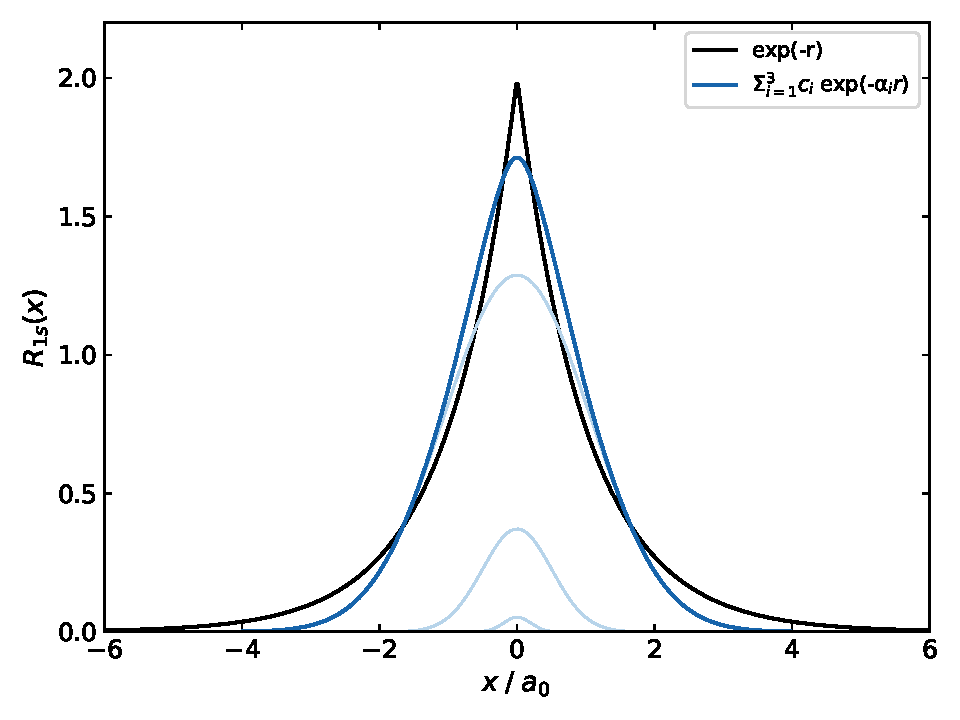
\includegraphics[width=11cm]{2/figs/fig1/gto_AO.pdf}
	\vspace{0.2cm}
	\hrule
	\caption{Exact (black line) and approximate (blue line) radial part of the hydrogen 1s orbital. Exponents and coefficients of primitive GTOs obtained from the def2-SVP basis set.\cite{BSE2019, Gulde2012}}
	\label{fig::gto_AO}
\end{figure}

For multielectron species a better approximation to the true AOs can be obtained using a combination of several STOs, themselves comprised of Gaussian primitives, as

\begin{equation}
	\phi_l^\text{AO}(\boldsymbol{x}_1) =  Y(\theta,\phi)[k_1 r^l \exp(-\zeta_1 r) + k_2 r^l \exp(-\zeta_2 r) + \cdots + k_n r^l \exp(-\zeta_n r)]
\end{equation}

for a $n$-$\zeta$ basis set with angular quantum number $l$. High kinetic energy close to nuclei means the curvature is important to the energy so several primitives are often combined for a single-$\zeta$, and fewer with multiple$-\zeta$ for valance electrons to form a 'split-valance' basis set.

With enough GTOs the AOs can be well approximated, but at a higher computational cost. Therefore, there is a balance between acceptable accuracy and cost in each calculation. DFT has the advantage of faster basis set convergence,\cite{Jan1995} with acceptable forces using a double-$\zeta$ quality basis and energies at triple-$\zeta$.\cite{Sure2015chemopen} WF methods are slower to converge with at least a triple-$\zeta$ basis set required for accurate energetics, with a CCSD(T) approximation energy differences are often within `chemical accuracy'.\cite{Zhang2012} Therefore, the split valance def2-SVP basis set will be used for geometry optimisations and the def2-TZVP (and variants thereof) for single point energy evaluations using both DFT and CC methods. These choices have been validated previously.\cite{Kirschner2020}

Two types of error emerge using finite basis sets: basis set incompleteness error (BSIE) and basis set superposition error (BSSE). The former is intrinsic for any calculation but particularly prominent when, for example, calculating anion energies without slowly decaying radial components (diffuse basis functions). The latter appears only when energy differences for association/dissociation processes are calculated, where one molecule can 'steal' basis functions from  another (often) lowering the energy more than would be expected at the basis set limit, thus artificially stabilising the complex.\footnote{Note that the distinction is somewhat arbitrary but BSIE is often taken to be the residual error to the complete basis set value once the BSSE has been corrected with a scheme. Both errors tend to zero at an infinitely large basis set.}\cite{BSSE1999}

The basis set size required for calculations of synthetically interesting molecules (10s-100s atoms) makes the formal scaling of DFT $O(N^3\mbox{--}N^4)$ and \emph{ab--initio} $O(N^{>4})$ too severe. Asymptotically, the scaling is reduced to $O(N^2)$ as the overlap between significantly separated AOs becomes negligible.\cite{Dyczmons1973} A resolution of the identity (RI) approximation builds on this to reduce the scaling to $O(N^2)$ for all system sizes by approximating two-electron integrals in an auxiliary basis.\cite{Hser1989} However, as most methods rely on a matrix diagonalisation, the scaling is only reduced to $O(N^3)$ if conventional (non-sparse) diagonalisation routines are employed. Multiple algorithms for implementing RI are available, with the chain-of-spheres (COS) for exact exchange terms being particularly efficient for large molecules.

% https://citeseerx.ist.psu.edu/viewdoc/download?doi=10.1.1.523.2841&rep=rep1&type=pdf
%http://www.tcm.phy.cam.ac.uk/~cks22/PAPER8/paper8.html

CCSD(T) calculations on large systems requires accelerations beyond RI in the Hartree-Fock step to combat the prohibitive $O(N^7)$ scaling. Most of these rely on the locality of electron correlation (i.e. local coupled cluster methods, LCC) to truncate the number of amplitudes included in the CC WF.\cite{Werner2011} Of particular note is the domain-based local pair natural orbital DLPNO method, which uses this truncation to approach a linear [$O(N^1)$] scaling method for CCSD,\cite{Riplinger2013} and perturbative triples.\cite{Yang2018}

\subsection{Periodic Electronic Structure}

Molecular finite size calculations allow gas phase or implicit-environment energies to be calculated. However, to include the environment explicitly without unphysical boundary effects would make the system size unmanageable. Periodic electronic structure calculations allow for a quasi-infinite system with repeated periodic images using, most commonly, DFT.\cite{Hasnip2014} Periodic DFT usually makes use of a `plane wave' basis set,

\begin{equation}
	\phi_{\boldsymbol{k}}^\text{PW}(\boldsymbol{r}_1) = \sum_{i, j} c_{i, j}\exp(\text{i}(\boldsymbol{k}_i + \boldsymbol{G}_j)\cdot \boldsymbol{r}_1)
\end{equation}

as a complex Fourier series, which satisfies translational symmetry, and is orthogonal. Here, $\text{i}$ is the imaginary unit, $\boldsymbol{k}$ a point in reciprocal space and $\boldsymbol{G}_i$ a quantised reciprocal lattice vector with $|\boldsymbol{k}_i + \boldsymbol{G}_i|^2/2 < E_\text{cut}$ for a cut-off PW energy of $E_\text{cut}$.\cite{DFTPracticalIntro2009} For sufficiently large super cells sampling just at the origin in $k$-space (the $\Gamma$-point) is sufficient.\cite{Kratzer2019}
 To overcome the intrinsically shallow curvature of plane waves a large $E_\text{cut}$ is required along with treating core electrons, with high kinetic energy, using pseudopotentials (PP). These PPs seek to replace the nuclear charge and thus diverging Coulomb attraction and the tightly-bound electrons with an effective ionic potential and are essential in periodic calculations. A similar strategy is employed in molecular systems for heavy elements (greater than period 4), where relativistic effects need to be included and are done so implicitly in effective core potentials (ECPs).

\subsection{Semi-empirical Methods}

For systems of more than a few hundred atoms the computational demands of DFT preclude its routine use. Semi-empirical methods on the other hand, sacrifice accuracy for speed and the ability to easily perform calculations with hundreds or thousands of atoms.\cite{Christensen2016} HF-derived methods including the PM$x$ (parametrisation method number $x$) family rely on several approximations:

\begin{enumerate}
	\item Only valance orbitals are included in the calculation (i.e. ECPs are employed for period 2 elements and above).
	\item Core-core repulsion is parametrised rather than the true Columb interaction between the nuclei.
	\item Two index electron repulsion integrals are parametrised.
	\item Atomic orbitals on different atoms are assumed to have no overlap.
\end{enumerate}

The most recent PM7 method makes use of the modified neglect of diatomic overlap (MNDO) method in which (1) two-electron integrals are approximated by a classical expansion of multipole moments (2) a dispersion correction is included and (3) adds a Gaussian repulsion between cores.

Tight binding (TB) DFT, in contrast, makes use of a Taylor expansion in the density and a minimal basis set to arrive at a general expression,

\begin{equation}
	E_\text{TB-DFT} = \sum_a f_a \sum_{i, j} c_i^a c_j^a H_{ij} + \sum_{A > B} \gamma_{AB}(R_{AB}) \Delta q_A \Delta q_B + \sum_{A > B} V_\text{rep}(R_{AB})
\end{equation}
where $f_a$ is the occupation number of MO $a$, $c_i$ is an atomic orbital coefficient, $H$ is the parametrised Hamiltonian matrix, $q$ are partial charges and $V_\text{rep}$ is a repulsive function depending on internuclear distances. This simple functional form for the energy is fast to evaluate but is highly parametrised, thus can be non-transferable.\cite{Gaus2011}

%,
%\begin{equation}
% 	E[\rho] = E_0 [\rho_0] + E_1 [\rho_0, (\delta \rho)]  + E_2 [\rho_0, (\delta %\rho)^2]   + \cdots
%\end{equation}
%https://arxiv.org/pdf/0910.5861.pdf
%where $\rho_0$ is the density of the isolated atoms and $\delta\rho$ is a small perturbation including the charge transfer. 

Recently, Grimme and co-workers have developed a variant of DFTB denoted GFN$x$-XTB,\cite{Grimme2017xtb} parametrised on elements up to radon, which has been successful in a variety of contexts including molecular geometries and non-covalent interactions. The GFN2-xTB method uses a minimal basis with polarisation without pair-specific parameters, making it more applicable than standard DFTB.

These methods are, however, not without their limitations. For example, employing a minimal basis set generally leads to exaggerated anion instability and limited polarisation.\cite{Addicoat2014} As such, quantitative predictions from derived energy differences are generally not possible.

\subsection{Implicit Solvent Models}

Without modification molecular electronic structure calculations are performed in an effective vacuum. Chemical reactions, however, are generally conducted in the condensed phase, e.g. solution, melt or on surface.\cite{Sievers2016} For non-polar reactions in apolar solution the solvent effect may be small,\cite{Rush2014} but for highly charged species the stabilisation of charge separation by the solvent is critical to obtaining even modest accuracy (error $< 10 \text{ kcal mol}^{-1})$).\cite{harvey2018Primer}

The most efficient method of including solvent effects is to model them implicitly, wherein the electronic Hamiltonian is modified to include effective point charges describing the solvent plus other contributions. Their aim is to calculate the solvation energy by splitting the free energy into electrostatic, cavitation, dispersion and repulsion terms as,\cite{Takano2004}
\begin{equation}
	\Delta G_\text{solv}(\text{solute}) = \Delta G_\text{ele} + \Delta G_\text{cav} + \Delta G_\text{disp} + \Delta G_\text{rep}
\end{equation}

In PCM and derivatives thereof (including CPCM) the electrostatic contribution involves interactions of point charges on the tessellated solute surface with a continuum model of the solvent (depending on its dielectric). The cavitation term depends on the spherical size of the solute and the number density of the solvent,  the repulsion just on the surface, while the dispersion uses an effective solute density matrix -- as in the SMD solvent model\cite{Marenich2009} -- or set of point charges.\cite{Tomasi2005}
 
% https://pubs.acs.org/doi/pdf/10.1021/acs.jctc.7b00169
% https://manual.q-chem.com/5.3/topic_solvation.html
% https://pubs.acs.org/doi/pdf/10.1021/cr00031a013

\subsection{Analysis Methods}

Once a calculation has been performed and an energy (difference) obtained, analysis methods can be used to try rationalise experimental energy differences. These are based on the density or molecular orbitals of the system with those pertinent to this thesis summarised in \figurename{ \ref{fig::intro_analysis_methods}} for a prototypical S$_\text{N}$2 reaction. 


\begin{figure}[h!]
	\centering
	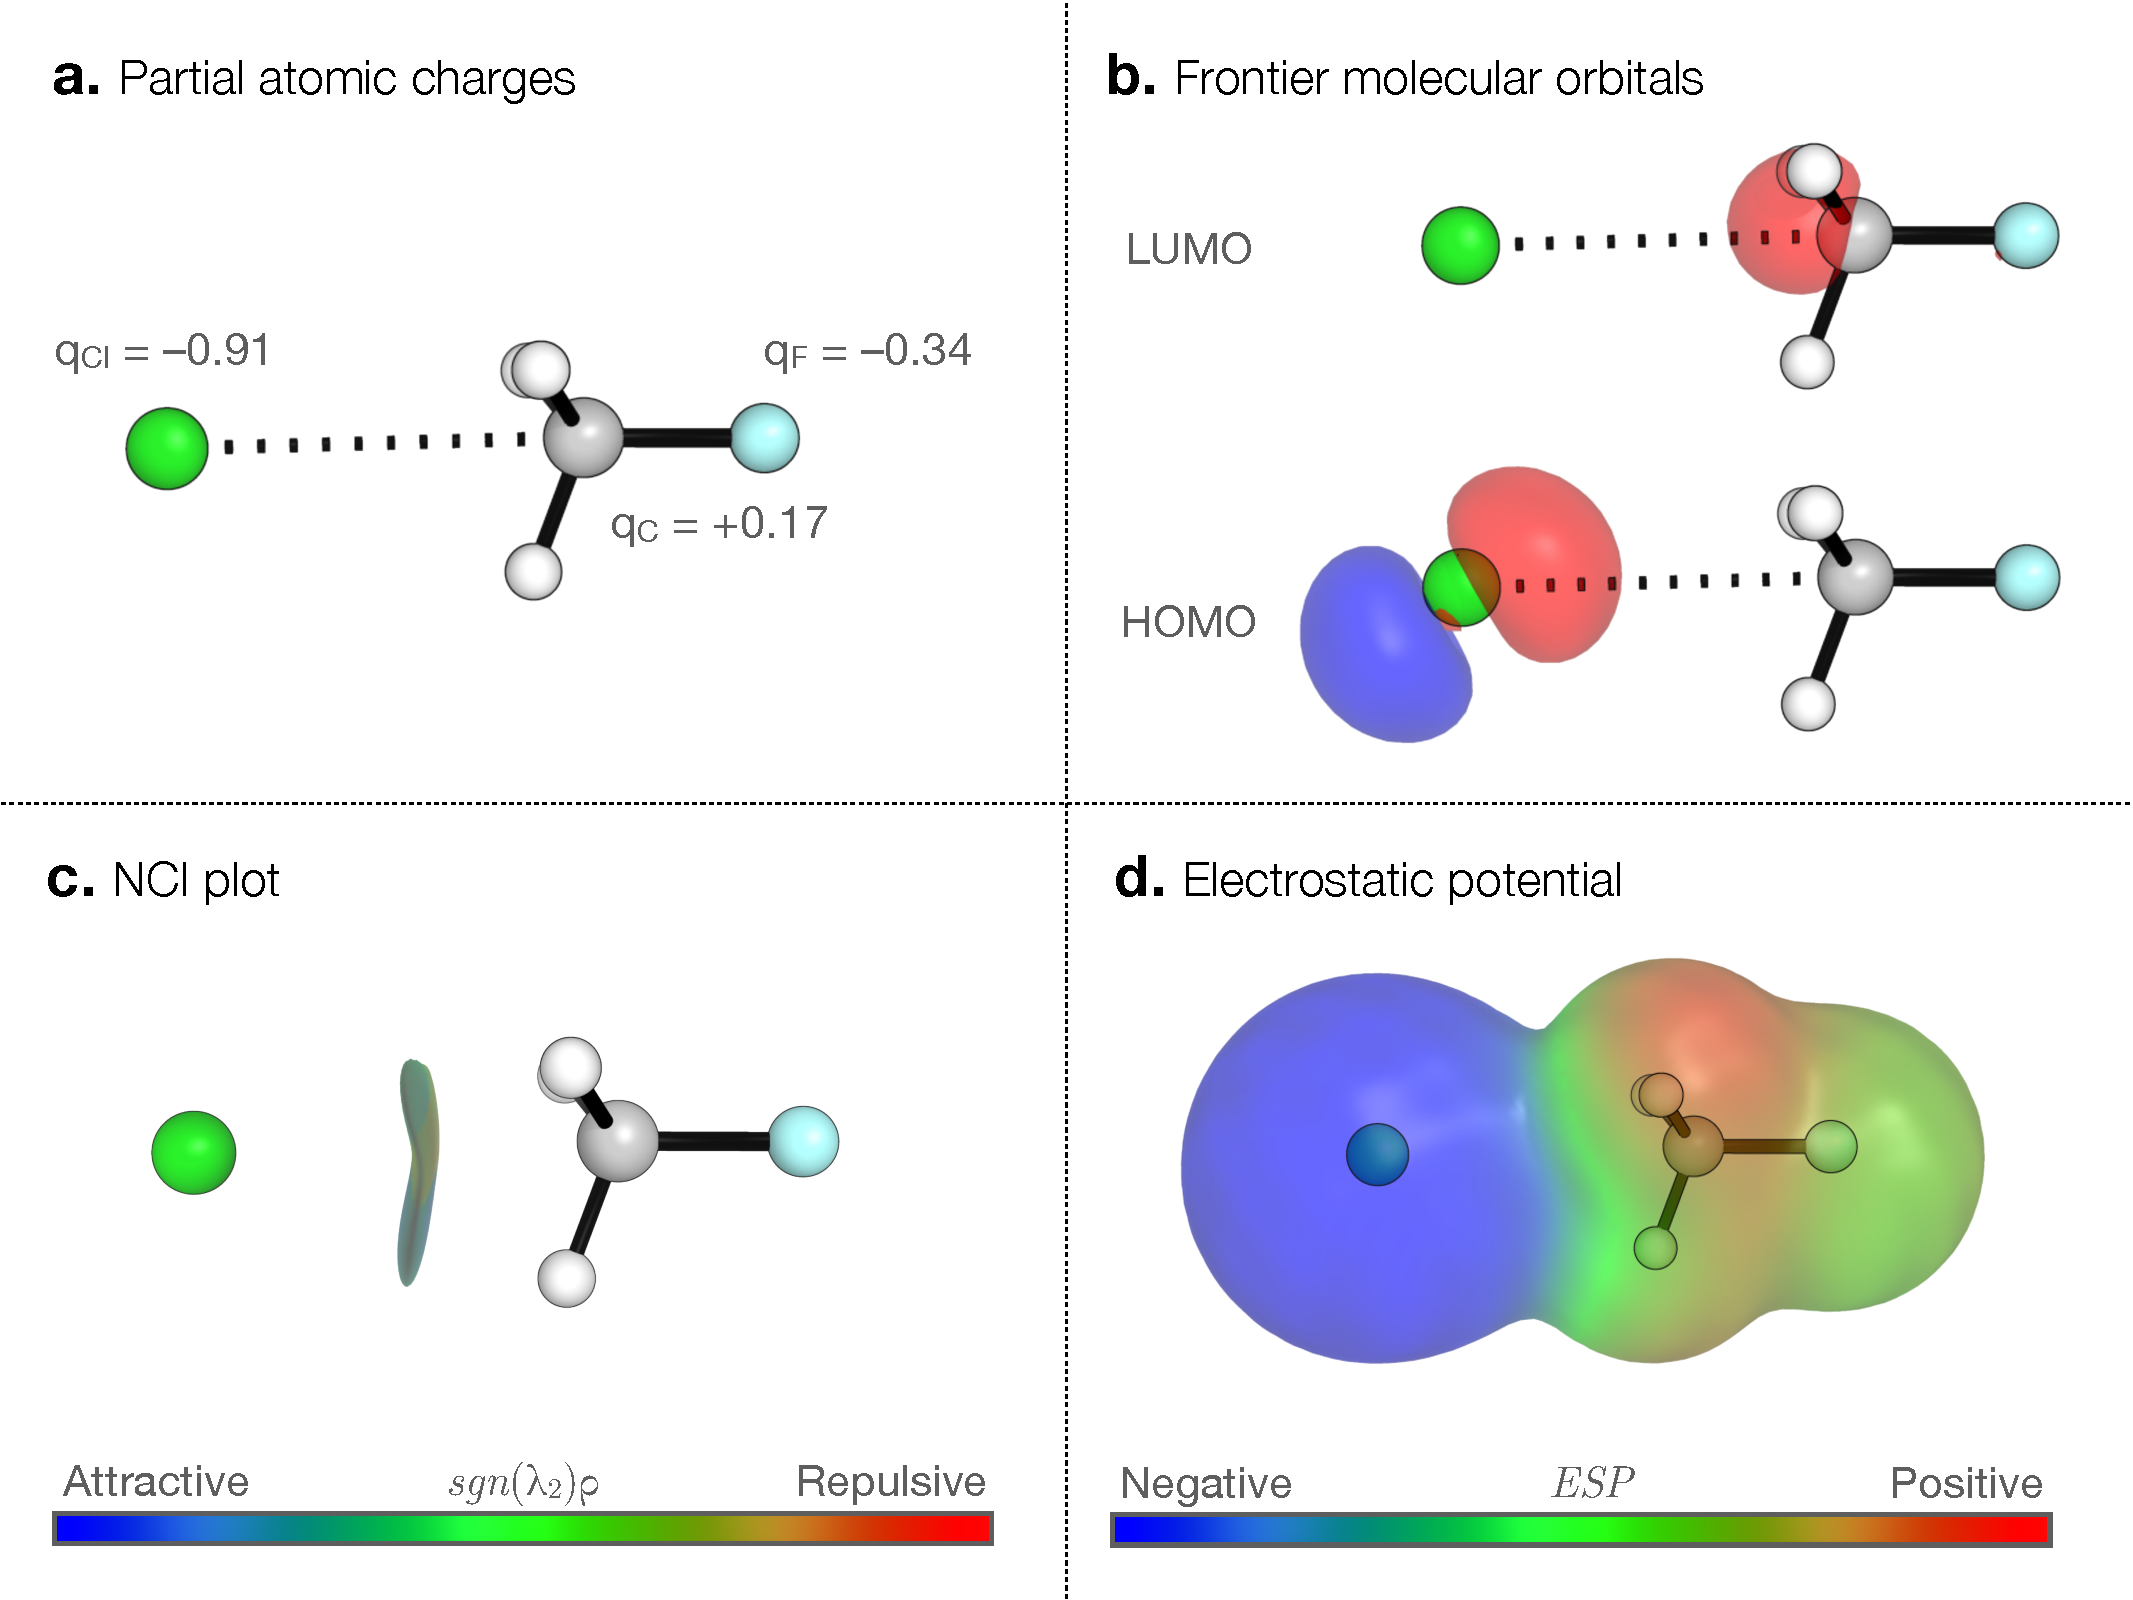
\includegraphics[width=\textwidth]{2/figs/fig2/analysis.pdf}
	\vspace{0.1cm}
	\hrule
	\caption{Electron density and orbital analysis methods applied to an S$_\text{N}$2 association complex Cl${}^{-}$.CH${}_3$F. DFT (SMD(water)-PBE0-D3BJ/def2-SVP) orbitals and corresponding density used in each case.}
		% ESP plotted over the range [-0.25, 0.0] Ha at a density isosurface of 0.002 $e/a_0^3$, non-covalent interaction (NCI) plot over [-0.02, 0.02]$e/a_0^3$ }
	\label{fig::intro_analysis_methods}
\end{figure}


\subsubsection{Partial atomic charges}

From a set of orbitals or a density, partial atomic charges may be defined and can provide useful chemical insights. For example, the atomic charges within the Cl${}^{-}$.CH${}_3$F association complex (\figurename{ \ref{fig::intro_analysis_methods}a}) suggest the flow of electron density from Cl$^{-}$ to C in the reaction.

As they are not observable quantities many schemes exist; the most simple being the Mulliken scheme, where an atomic charge on an atom $A$ is defined as,\cite{SzaboIntro}
\begin{equation}
	q_A = Z_A - \sum_{\mu \in A} (\boldsymbol{P}\boldsymbol{S})_{\mu \mu}
\end{equation}
where $\boldsymbol{P}$ and $\boldsymbol{S}$ are density and overlap matrices respectively (in the AO basis) and the sum is over orbitals centred on atom $A$. However, the basis set dependence of Mulliken partial charges is significant,\cite{Cusachs1968} and so have been superseded by other schemes. Hirshfeld charges are derived from the density and converge as the basis set increased in particular,\cite{Hirshfeld1977}
\begin{equation}
	q_A = Z_a - \int w_A(\boldsymbol{x}) \rho^\text{mol}(\boldsymbol{x}) - \rho^\text{atom}_A(\boldsymbol{x}) \;\text{d}\boldsymbol{x}
\end{equation}

where $w_A$ is a weighting function defined by $w_A = \rho_A^\text{atom}/\sum_B \rho_B^\text{atom}$ and $\rho_A^\text{atom}$ is the isolated atomic density of atom $A$. Although sensitive to the choice of reference atomic density, the trends between systems are generally considered to be robust compared to basis-set dependent schemes.\cite{Saha2008}

	% Orbtial methods
	% Hirshfield
	
\subsubsection{Frontier molecular orbital theory}

While not physical observables, frontier canonical orbitals -- those close in energy to the first unoccupied -- can be predict where a reaction will occur.\cite{Fukui1952, Woodward1969, Fukui1982} Interaction between the highest occupied MO (HOMO) and lowest unoccupied MO (LUMO) can lead to a stabilising interaction,\cite{albright2013orbital} and used to rationalise attractive interactions. For example, types of halogen bonding (B$\rightarrow$X--E, where B is a base, X a halogen and E another element) may be attributed to a $n\rightarrow \sigma^*$ interaction, where high-lying filled MO has lone pair ($n$)-like character and a low-lying unoccupied orbital is a $\sigma^*$ orbital.\cite{Cavallo2016} Pictorially, \figurename{ \ref{fig::intro_analysis_methods}b} shows the HOMO of Cl${}^{-}$.CH${}_3$F as a chloride lone pair that can `donate into' the LUMO as a $\sigma^*$ of the C--F bond, thus suggesting the classic backside attack in the S${}_\text{N}2$ reaction.

\subsubsection{Non-covalent interactions}

The identification of non-covalent interactions (NCIs) may be located quantitatively using the reduced density gradient (RDG),\cite{Johnson2010}
\begin{equation}
	\text{RDG}(\boldsymbol{x}) \propto \frac{|\nabla \rho(\boldsymbol{x})|}{\rho(\boldsymbol{x})^{4/3}}
\end{equation}
which is the normalised magnitude of the density gradient. This definition affords moderate $\text{RDG}(\boldsymbol{x})$ with low densities but smaller values at higher density, such as within a chemical bond. Attractive interactions (e.g. H-bonds) have $\sgn(\lambda_2)\rho(\boldsymbol{x})  < 0$, while repulsive (steric clash) have $\sgn(\lambda_2)\rho(\boldsymbol{x}) > 0$, where $\lambda_2$ is the second largest eigenvalue of the Hessian matrix of the density and measures the charge accumulation in the perpendicular plane of the interaction.\cite{Laplaza2020} In the Cl${}^{-}$.CH${}_3$F association complex there is a moderate attractive interaction between the chloride and the slightly positively charged carbon (\figurename{ \ref{fig::intro_analysis_methods}c}), as would be expected.


\subsubsection{Electrostatic potential}

An electrostatic potential (ESP, $\Phi(\boldsymbol{x})$) is defined as the work required to add a unit positive charge at a point $\boldsymbol{x}$. In a molecule,

\begin{equation}
	\Phi(\boldsymbol{x}) = \sum_A \frac{Z_A}{|\boldsymbol{R}_A - \boldsymbol{x}|} - \int \frac{\rho(\boldsymbol{x'})}{|\boldsymbol{x'} - \boldsymbol{x}|} \text{d}\boldsymbol{x}' \;\approx\; \sum_A \frac{q_A}{|\boldsymbol{R}_A - \boldsymbol{x}|}
\end{equation}

where the sum runs over nuclei $A$. Plotting the ESP over a molecular surface (e.g. Van der Walls, using some radii) allows for the rapid identification of areas of charge accumulation and where, for example, hydrogen bonds are likely to form.\cite{Politzer2001} For example, the ESP of Cl${}^{-}$.CH${}_3$F over a density isosurface is shown in \figurename{ \ref{fig::intro_analysis_methods}d}, clearly showing the location of the negative charge `located' on Cl${}^{-}$.


\section{Molecular Dynamics}
\subsection{Preamble}
So far the methods outlined above have focused on calculating energies and analysing compounds at zero temperature at a single geometry. However, sampling of a system's potential energy surface (PES, $E(\boldsymbol{R})$) is essential to obtain observable properties. In the most simple case, the sampling corresponds to a geometry optimisation; where from a single point, optimisation affords a stationary point on the hypersurface at which energies may be calculated. 

Sampling more than just a set of points en-route to a stationary point is sometimes essential. Most molecules can exist in multiple conformations, disregarding some of which may lead to incorrect reaction energetics.\cite{Hawkins2017} Moreover, considering only stationary points can be a severe approximation, as chemistry is conduced at non-zero temperatures where nuclei can move. To calculate free energies and sample from the correct ensembles requires dynamics. For example, in free energy perturbation (FEP)  theory the difference is given by the Zwanzig equation,
\begin{equation}
	\Delta F_{\text{X}\rightarrow\text{Y}} = -R T \left\langle \exp\left( - \frac{E_\text{Y} - E_\text{X}}{RT} \right) \right\rangle_\text{X}
	\label{equation::zwanzig}
\end{equation}

where $R$ is the gas constant, $T$ the temperature, $F$ a free energy (Helmholtz or Gibbs) and the angle brackets indicate an ensemble average over state X. A Helmholtz free energy ($A$) is defined within an $NVT$ ensemble where the number of particles ($N$), volume ($V$) and temperature is constant, while the Gibbs free energy replaces constant volume with pressure $NPT$ ensemble.

The average in \eqref{equation::zwanzig} may be computed using molecular dynamics (MD), or Monte Carlo (MC, e.g. Metropolis Monte Carlo) both of which \emph{can} sample from the correct ensembles.


\subsection{Integration Algorithms}

MD simulations require propagating equations of motion forwards using the energy and curvature of the PES. This may be using quantum mechanics, but is prohibitively expensive for large molecules ($\gtrsim$10 atoms).\cite{Zhang2016} Classical MD is, therefore, the choice method for sampling, where Newton's equations of motions ($\boldsymbol{F}=\boldsymbol{m}\boldsymbol{a}$) are integrated with, for example, a velocity Verlet algorithm for updated positions and velocities,


\begin{equation}
	\begin{aligned}
		\boldsymbol{R}(t+\Delta t) &= \boldsymbol{R}(t) + \boldsymbol{v}(t) \Delta t + \frac{\boldsymbol{F}(t) }{2 \boldsymbol{m}} (\Delta t)^2\\
		\boldsymbol{v}(t + \Delta t) &= \boldsymbol{v}(t)  + \frac{\boldsymbol{F}(t) + \boldsymbol{F}(t+\Delta t)}{2\boldsymbol{m}} \Delta t
	\end{aligned}
\end{equation}

for a collection of nuclear coordinates $\boldsymbol{R}$ with velocities $\boldsymbol{v}$, masses $\boldsymbol{m}$ and forces $\boldsymbol{F}$. This just corresponds to a Taylor expansion in the position and velocities, and the velocity update uses the average of the force between the current step and the next.

Iterating these equations requires a time-step ($\Delta t$) small enough for the expansion to be accurate but large enough to be computationally efficient. In practice, this is chosen to be $\sim 1$ fs and corresponds to the fastest motion (bond stretching), while fixing E-H bonds allows for a larger 2 fs time-step.\cite{Sweet2013}

In a closed $NVT$ ensemble the energy is conserved, thus the temperature $T \sim 2 T_\text{KE} / 3Nk_\text{B}$ (for $N$ particles) fluctuates as the system accesses different regions of the PES. To simulate at constant temperature  requires thermostats.

\subsection{Thermostats}

Constant simulation temperature can be achieved using stochastic; strong or weak coupling methods; additional degrees of freedom to the system can also be added. Langevin dynamics makes use of a velocity damping along with stochastic Gaussian random noise with an equation of motion,
\begin{equation}
	\ddot{\boldsymbol{R}}(t) = \frac{\boldsymbol{F}}{\boldsymbol{m}} - \gamma \boldsymbol{v}(t) + \sqrt{\frac{2\gamma k_\text{B} T}{\boldsymbol{m}}} \vartheta(t)
\end{equation}
where $\gamma$ is a damping parameter and $\vartheta(t)$ a stationary distribution with zero mean and zero covariance with any other time. From the strong coupling thermostats the velocity rescale thermostat in its most simple form multiplies all the velocities by a factor $\alpha = \sqrt{\bar{T}_\text{KE} / T_\text{KE}}$, where $\bar{T}_\text{KE}$ is the desired kinetic energy given a temperature.\cite{Bussi2007} As most condensed phase molecular systems undergo little volume change through reactions etc. constant pressure simulations (NPT) will not be discussed; likewise for unconstrained particle number simulations. 

\subsection{Empirical Force Fields}

With equations of motion to propagate for sampling within an ensemble depending on forces, a method of calculating them efficiently is required. While QM methods (DFT, MP2 etc.) can be used to calculate forces, often many thousands of gradient evaluations are required and can be too computationally demanding. Collectively known as \emph{ab initio} molecular dynamics (AIMD) is generally only suitable for sampling on picosecond timescales.\cite{Iftimie2005} To calculate forces efficiently and access timescales of nano or microseconds requires a parametrisation of the PES. Empirical force-fields for molecular systems rely on a bonded + non-bonded decomposition of the energy,

\begin{equation}
	E_\text{FF} = E_\text{bonded} + E_\text{non-bonded}
\end{equation}
where the respective terms usually have the form,
\begin{equation}
	E_\text{bonded} = \underbrace{\sum_{i, j}^\text{bonds} k_{ij} (r_{ij} - r_{ij}^0)^2}_\text{bond stretching} + \underbrace{\sum_{i, j, k}^\text{angles} k^\theta_{ijk} (\theta_{ijk} - \theta_{ijk}^0)^2}_\text{angle bending} + \underbrace{\sum_{m}^\text{dihedrals} k_m (1 + \cos(n^m \chi_m - \mu^m))}_\text{dihedral rotation}
\end{equation}
for distances ($r$), angles ($\theta$) and dihedrals ($\chi$)\footnote{Improper dihedrals between four non-contiguous atoms employ a harmonic term but are omitted for clarity.} where superscript 0 denotes an equilibrium value while $i,j,k$ enumerate over atoms $m$ over dihedrals, $n$ is an integer while $\mu$ is a shift factor. The non-bonded component often takes the form of a Lennard-Jones term for dispersion and repulsion, and an electrostatic monopole interaction,

\begin{equation}
	E_\text{non-bonded} = \sum_{i, j}^\text{pairs} \; \underbrace{\epsilon_{ij} \left( \left(\frac{\sigma_{ij}}{r_{ij}}\right)^{12} - \left(\frac{\sigma'_{ij}}{r_{ij}}\right)^6 \right)}_\text{LJ 12-6 potential} + \underbrace{\frac{q_i q_j}{r_{ij}}}_\text{electrostatic}
\end{equation}

where $\epsilon$ is proportional to the well depth and $q$ a partial atomic charge.\cite{Guvench2008} In combination with neighbour lists the complexity scales as roughly $O(N)$ for large systems and, because only simple mathematical operations are required, the execution is rapid. While minimal, this type of description is employed in almost all classical biomolecular MD simulations.\cite{Schlick2021}

This description of the PES is, however, not without its limitations, particularly important are: (1) bonds are harmonic and cannot break, making reactive events impossible to study; (2) static charges are used with no polarisation/charge transfer possible; (3) dispersion is not pairwise additive; (4) closed shell repulsion is exponential in distance not $r^{-12}$; (5) angle potentials are fully harmonic and cannot have two minima (e.g. trigonal bi-pyramidal and square planar metal complexes); (6) fixed atom types are used to define $\epsilon, \sigma$ for a pair of atoms using combination rules, which are an approximation to the optimum values.\cite{Boda2008} Therefore, employing these empirical potentials requires consideration of the resulting (somewhat unknowable) errors, potential lack of transferability and may not facilitate in quantitative comparisons.\cite{Harrison2018, LewisAtwell2021}


\section{Machine Learnt Potentials}
\subsection{Preamble}

Machine learning concerns the development and study of computer algorithms that improve with data.\cite{Mitchell1997} Categorised into supervised and unsupervised flavours depending on whether the target values are known or not, ML has been widely adopted in the sciences since its inception in  the 1960s.\cite{Carleo2019} Within the chemical domain applications include advanced quantitative structure activity relationships (QSAR) and interatomic potentials (ML force-fields), amongst many others.\cite{Cova2019} An ML or 'data-driven' approach to a potential may be written as,
\begin{equation}
	E(\boldsymbol{R}) = f(\boldsymbol{R}; \boldsymbol{\alpha})
\end{equation}
where the potential energy $E$ is given by a function (the ML potential) of the systems' nuclear coordinates and a set of parameters ($\boldsymbol{\alpha}$). The parameters are obtained using a set of prior observations $\{\boldsymbol{R}_\text{train}\}$ and output labels $\{E_\text{train}\}$ with, perhaps, forces ($\{-\partial E_\text{train}/\partial R_i\}$). Exhaustively generating points in the space is, however, in for more than a few atoms as $M^{3N_\text{atoms}}$ points are needed for a grid over the whole space with $M$ points in each dimension. To somewhat aliviate the exponential scaling, generally the total energy is generally written as a sum of atomic contributions as,

\begin{equation}
	E(\boldsymbol{R}) = \sum_i^\text{atoms} f_i (\boldsymbol{R}_i; \boldsymbol{R}_{\ne i}, \tilde{\boldsymbol{\alpha}})
\end{equation}

where now the atomic energy given by $f_i$ depends on its position ($\boldsymbol{R}_i$), and of those atoms around it (within some cut-off) along with a set of parameters. With this atomic expansion of the energy, which is assumed to be possible, the space to fit is much smaller if the cut-off does not include the whole system and symmetries in the system can be exploited.\footnote{Two well separated water molecules, for example are essentially non-interacting thus the energy is a simple sum of the two components.}

\subsection{Representations}

To minimise the quantity of data required to obtain a ML potential at some accuracy requires encoding all the relevant symmetries into a `representation' i.e. $\boldsymbol{R} \mapsto \boldsymbol{R}_F$ for a feature vector $\boldsymbol{R}_F$. The vector $\boldsymbol{R}_F$ should be invariant to translation, rotation and permutation of like nuclei, as the Hamiltonian is invariant to all of those operations.

The initial work of Behler and Parrinello showed that PES fitting using ML approaches was possible using artificial neural networks (ANNs, or NNs) and employed atomic-centred symmetry functions (ACSF).\cite{Behler2007, Behler2011} While many possible radial and angular functions were proposed the most frequently employed is a set of shifted Gaussian functions as,

\begin{equation}
	G^{R_s, \eta}_i(\boldsymbol{R}) = \sum_j^\text{neighbours} \exp\left[-\eta (R_{ij}- R_s)^2 \right] f_c({R_{ij}})
	\label{equation::behler_acsf}
\end{equation}

where $R_{ij} = |\boldsymbol{R}_i - \boldsymbol{R}_j|$, $\eta, R_s$ are parameters and $f_c(R_{ij}) = 0.5[\cos(\pi R_{ij} / R_c) + 1]$ for $R_{ij} < R_c$ and zero otherwise, given a cut-off distance $R_c$. The cut-off function ($f_c$) ensures a zero output outside of the cut-off region such that the derivatives are continuous. A similar function to Eqn. 
\eqref{equation::behler_acsf} is defined for angular components using a cosine function damped with Gaussians and cut-off functions. Concatenating elements of radial and angular functions with varying parameters affords $\boldsymbol{R}_F$. These functions and their variants have been used extensively in bespoke and general (e.g. ANI\cite{Smith2017}) machine learnt potentials.

 % https://pubs.rsc.org/en/content/articlepdf/2017/sc/c6sc05720a
%https://aip.scitation.org/doi/pdf/10.1063/1.3553717


Alternatively, an atomic environment may be expressed using an effective atomic density and $\boldsymbol{R}_F$ constructed from the set of expansion coefficients of that density, as in the smooth overlap of atomic positions (SOAP) descriptor.\cite{Bartok2013} Specifically, for an atomic neighbour density,
\begin{equation}
	\rho_i(\boldsymbol{x}) = \sum_j^\text{neighbours} w_i \delta(\boldsymbol{x} - \boldsymbol{R}_j)
\end{equation}

with a set of weights $w_i$, $\boldsymbol{x}$ is a position in space centred at $\boldsymbol{R}_i$, and $\delta$ a Dirac delta centred on each neighbouring atom. To ensure the descriptor is smooth under coordinate perturbations Gaussians are used in place of the delta functions and the density expanded in a radial $g$ and spherical harmonic $Y$ basis as,
\begin{equation}
	\rho_i(\boldsymbol{x}) = \sum_j^\text{neighbours}  \exp(-\sigma_\text{atom} |\boldsymbol{x} - \boldsymbol{R}_j|^2)  = \sum_{nlm} c_{nml} g_n(r) Y_{lm}(\theta, \phi)
\end{equation}

where $\sigma_\text{atom}$ controls the atomic density extent. See Appendix \ref{section::soap_derivation} for a derivation of the coefficients. The SOAP vector is then defined from the power spectrum elements as
\begin{equation}
	\boldsymbol{p}_i = \{p_{n n' l}\} \qquad ; \qquad p_{n n' l} = \frac{1}{\sqrt{2l + 1}} \sum_{m=-l}^l c_{nlm}^* c_{n'lm}
\end{equation}

to afford a rotationally-invariant description of the neighbour density of atom $i$, schematically shown in \figurename{ \ref{fig::theory_soap}}.

\begin{figure}[h!]
	\centering
	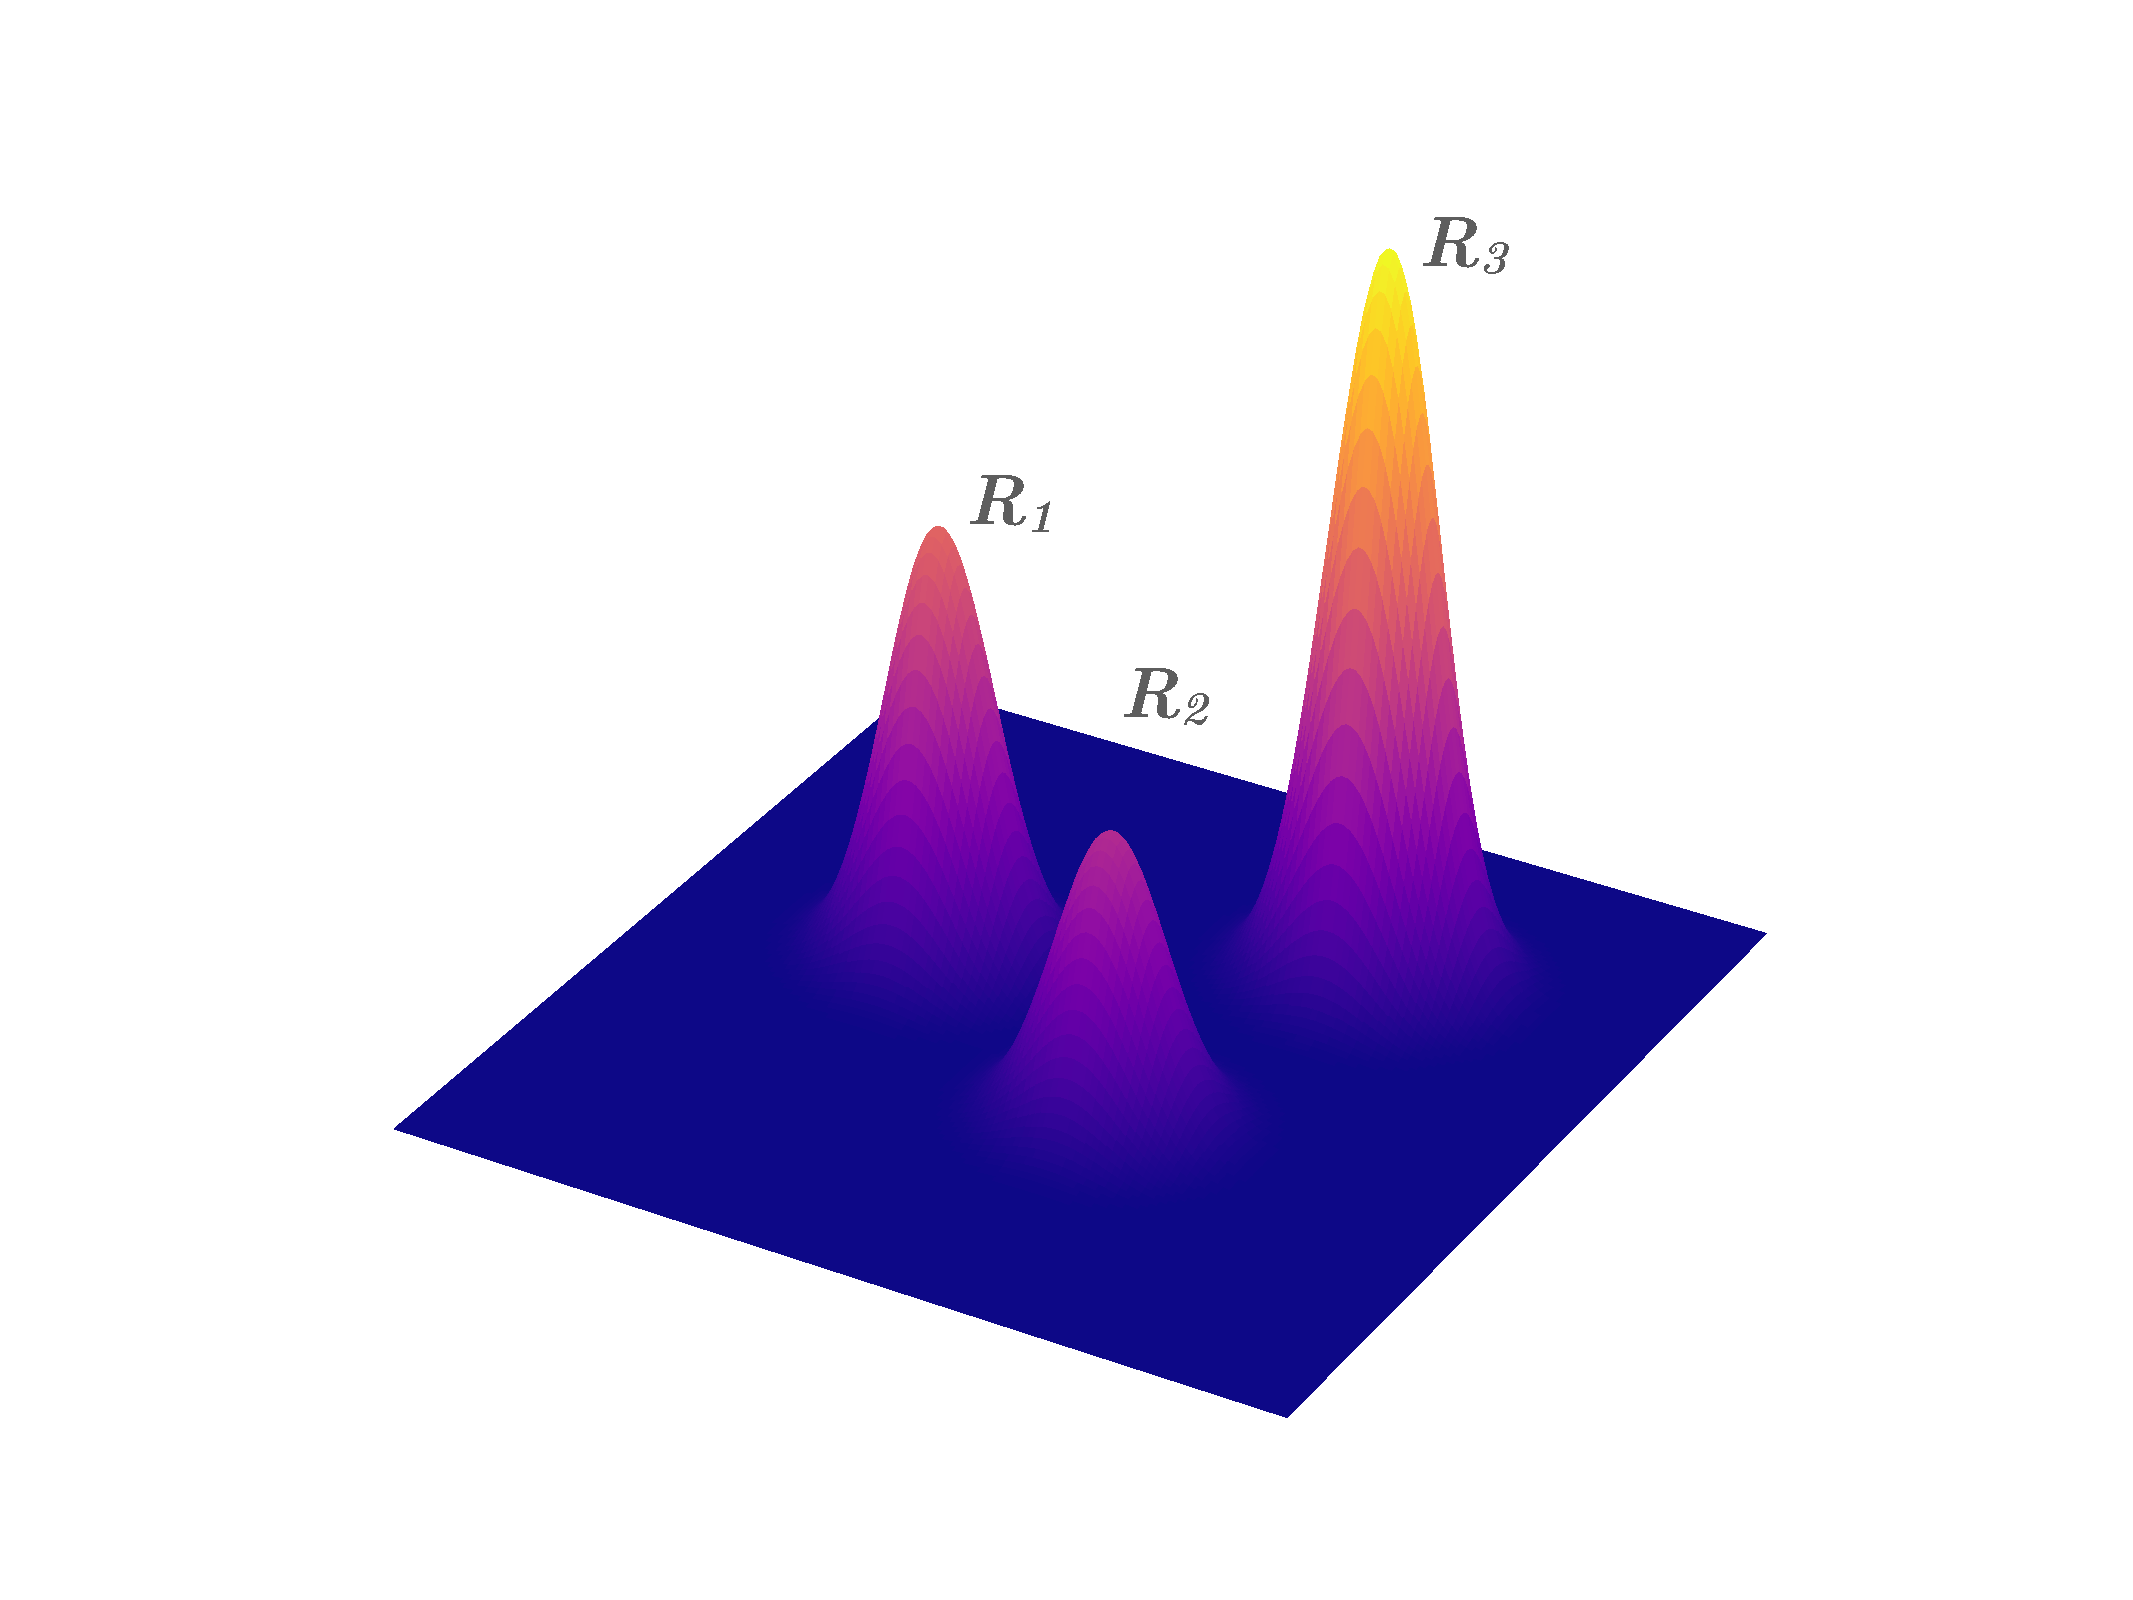
\includegraphics[width=9cm]{2/figs/fig3/SOAP.pdf}
	\vspace{0.5cm}
	\hrule
	\caption{Smooth overlap of atomic positions density of three neighbours with differing weights.}
	\label{fig::theory_soap}
\end{figure}


 Using the default parametrisations both ACSFs and the SOAP power spectrum seem to perform similarly at representing atomic environments.\cite{Pozdnyakov2020, Onat2020} The choice of atomic description amongst the wide variety (also including Chebyshev polynomials\cite{Thompson2015}, many-body tensor representation\cite{Huo2018unified}, permutationally invariant polynomials\cite{Braams2009, Oord2020}, amongst others) is then just dependent on the implementation and computational efficiency.

% https://aip.scitation.org/doi/pdf/10.1063/5.0016005

\subsection{Regression Algorithms}

From a compact and representative $\boldsymbol{R}_F$ an atomic energy prediction is made using a regression algorithm. Of the wide variety (linear, polynomial, support vector machine (SVM), decision trees etc.\cite{HandsOnML2019}) ANNs and Gaussian process regression (GPR) are the most widely employed,\cite{Mueller2020} and so are briefly outlined below.

A simple 'feed-forward' neural network consists of a set of layers, each containing nodes which transform an input $x$ as,
\begin{equation}
	y = \sigma(w x + b)
\end{equation}
where $w$ is a weight and $b$ a bias, and $\sigma$ an activation function e.g. $\sigma = \tanh$ is generally introduced to apply a non-linear transform enabling a ANN to approximate any function.\cite{Nielsen2015neural} Introducing $n$ layers each with multiple nodes the output is,
\begin{equation}
	y = \sigma_n \circ \cdots \circ \sigma_1(\boldsymbol{w}_1 \boldsymbol{X} + \boldsymbol{b}_1)
\end{equation}
where at each layer the input $\boldsymbol{X} \in \mathbb{R}^{N_\text{in}}$, $\boldsymbol{b} \in \mathbb{R}^{N_\text{out}}$ and $\boldsymbol{w} \in \mathbb{R}^{N_\text{out} \times N_\text{in}}$ is a weight matrix with $\circ$ denoting function composition. The weights and biases are then optimised by minimising a smooth loss function [$L(y, y_\text{target})$] with respect to the parameters over many target values within a `batch'. 

Gaussian process regression starts by defining the output in a linear way,
\begin{equation}
	y = \sum_i w_i \phi_i(\boldsymbol{X})
\end{equation}
where again $w$ are weights but now $\phi$ defines a basis function. By using weights initialised from Gaussians with zero mean an variance, a new value can be predicted at its mean,\cite{Bartok2015, Williams1996gaussian}
\begin{equation}
	y^* = \boldsymbol{k}^T(\boldsymbol{X}^*) K^{-1} \boldsymbol{y}
\end{equation}
where $ \boldsymbol{k}^T(\boldsymbol{X}^*) = (k(\boldsymbol{X}_1, \boldsymbol{X}^*), ..)$ and $K$ is the kernel matrix with elements $K_{ij} = k(\boldsymbol{X}_i, \boldsymbol{X}_j),$ and $\boldsymbol{y}$ a column vector of target values for each $\boldsymbol{X}$. In the context of a machine learnt potential i.e. a Gaussian approximation potential (GAP) the observations are total energies\footnote{Atomic forces can also be used as additional labels and, almost always, improve the fit.} and $\boldsymbol{X} = \boldsymbol{R}_F$ with the canonical SOAP kernel having elements
\begin{equation}
	k(\boldsymbol{X}_i, \boldsymbol{X}_j) = \sigma_w^2 \int_\text{space} \rho_i (\boldsymbol{x}) \rho_j (\boldsymbol{x})\; \text{d}\boldsymbol{x} = \sum_{n, n', l} p_{nn'l}^{(i)}p_{nn'l}^{(j)} 
\end{equation}

which just measures the similarity between two atomic neighbour densities, such that similar environments have kernel values close to one and, thus, likely similar energies. GAP implementations may also include two and three-body components such that the total energy is then a sum of terms and usually a radial basis function kernel,
\begin{equation}
	k_\text{RBF}(\boldsymbol{X}_i, \boldsymbol{X}_j) = \exp\left(-\frac{|\boldsymbol{X}_i - \boldsymbol{X}_j|}{2\theta^2}\right)
\end{equation}
where $\theta$ controls the interpolation range and $\boldsymbol{X}_i = d_i$ is the pairwise distance in a two-body descriptor.

With generally fewer parameters to define a GAP than an ANN they are the choice method for sparse datasets, but the evaluation scales (without other approximations) as $O(N^3)$ for $N$ training points due to the matrix inversion.





\clearpage
\end{document}